% ------------------------------------------------------------------------------
% TYPO3 Version 10.3 - What's New (Italian Version)
%
% @license	Creative Commons BY-NC-SA 3.0
% @link		https://typo3.org/help/documentation/whats-new/
% @language	Italian
% ------------------------------------------------------------------------------

\section{Introduzione}
\begin{frame}[fragile]
	\frametitle{Introduzione}

	\begin{center}\huge{Introduzione}\end{center}
	\begin{center}\huge{\color{typo3darkgrey}\textbf{I fatti in breve}}\end{center}

\end{frame}

% ------------------------------------------------------------------------------
% TYPO3 Version 10.3 - The Facts

\begin{frame}[fragile]
	\frametitle{Introduzione}
	\framesubtitle{TYPO3 Versione 10.3 - I fatti in breve}

	\begin{itemize}
		\item Data di rilascio: 25 Febbraio 2020
		\item Tipo di rilascio: Sprint Release
	\end{itemize}

	\begin{figure}
		
\includegraphics[width=0.95\linewidth]{Introduction/typo3-v10-3-banner.png}
	\end{figure}

\end{frame}

% ------------------------------------------------------------------------------
% TYPO3 Version 10.3 - Executive Summary

\begin{frame}[fragile]
	\frametitle{Introduzione}
	\framesubtitle{Sintesi}

	\small
		Come ultima versione del ciclo di rilasci sprint della v10, TYPO3 versione 10.3 è definita versione
		"\href{https://typo3.org/article/land-ho-feature-freeze-ahead}{feature freeze}".
		Questo significa nessuna nuova funzionalità d'ora in poi e fino alla versione LTS di aprile
		il core team e tutti i collaboratori saranno focalizzati sui test, la pulizia e
		il miglioramento della versione.

		\vspace{0.2cm}

		Tuttavia, ci possono essere alcune piccole eccezioni per il miglioramento delle funzionalità che sono
		già state aggiunte nelle precedenti versioni sprint della v10.

		\vspace{0.2cm}

		Se sei uno sviluppatore di estensioni pubblicale con versioni compatibili alla v10.
		Ciò renderà più semplice per la community TYPO3 l'adozione di TYPO3 v10 non appena
		sarà lanciata la versione LTS.

		\vspace{0.2cm}

		Un'ultima cosa importante: non dimenticare di unirti a un
		\href{https://typo3.org/community/events/v10-parties}{release party}
		o organizzarne uno tu stesso!

	\normalsize

\end{frame}

% ------------------------------------------------------------------------------
% System Requirements

\begin{frame}[fragile]
	\frametitle{Introduzione}
	\framesubtitle{Requisiti di sistema}

	\begin{itemize}
		\item PHP versione 7.2, 7.3 o 7.4
		\item Impostazioni PHP:

			\begin{itemize}
				\item \texttt{memory\_limit} >= 256M
				\item \texttt{max\_execution\_time} >= 240s
				\item \texttt{max\_input\_vars} >= 1500
				\item l'opzione di compilazione \texttt{-}\texttt{-disable-ipv6} \underline{non} deve essere usata
			\end{itemize}

		\item La maggior parte dei database supportati da \textbf{Doctrine DBAL} funzionano anche con TYPO3.
			I DB verificati sono ad esempio:
	\end{itemize}

	\begin{figure}
		
\includegraphics[width=0.80\linewidth]{Introduction/logo-databases.png}
	\end{figure}

\end{frame}

% ------------------------------------------------------------------------------
% Development, Release, and Maintenance Timeline

\begin{frame}[fragile]
	\frametitle{Introduzione}
	\framesubtitle{Sviluppo, tempi di rilascio e mantenimento}

	\textbf{TYPO3 v10}

	\begin{figure}
		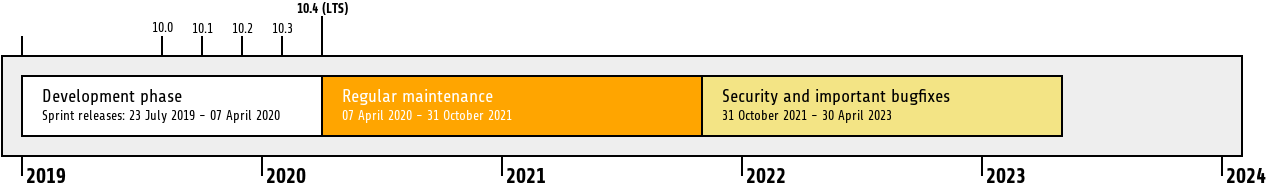
\includegraphics[width=1\linewidth]{Introduction/typo3-v10-lifecycle.png}
	\end{figure}

	\textbf{Supporto esteso}\newline
	\smaller
		La \href{https://typo3.com}{TYPO3 GmbH} offre ulteriori opzioni di supporto
		per TYPO3 v10 LTS anche dopo il 30 Aprile 2023, per ulteriori due anni.
	\normalsize

\end{frame}

% ------------------------------------------------------------------------------
% TYPO3 v10 Roadmap

\begin{frame}[fragile]
	\frametitle{Introduzione}
	\framesubtitle{TYPO3 v10 Roadmap}

	Date di rilascio e loro obiettivi principali:

	\begin{itemize}

		\item v10.0 \tabto{1.1cm}23/Lug/2019\tabto{3.4cm}Preparare la strada per nuovi concetti e API entusiasmanti
		\item v10.1 \tabto{1.1cm}01/Ott/2019\tabto{3.4cm}Miglioramenti nel routing e nel gestore di sito v2
		\item v10.2 \tabto{1.1cm}03/Dic/2019\tabto{3.4cm}Miglioramenti al motore di rendering Fluid
		\item
			\begingroup
				\color{typo3orange}
				v10.3 \tabto{1.1cm}25/Feb/2020\tabto{3.4cm}Conferma della funzionalità
			\endgroup
		\item v10.4 \tabto{1.1cm}21/Apr/2020\tabto{3.4cm}Rilascio LTS (Long-term Support)

	\end{itemize}

	\vspace{0.6cm}
	\smaller
		\url{https://typo3.org/article/typo3-v10-roadmap/}\newline
		\url{https://typo3.org/article/typo3-v10-safe-and-sound/}
	\normalsize

\end{frame}

% ------------------------------------------------------------------------------
% Installation

\begin{frame}[fragile]
	\frametitle{Introduzione}
	\framesubtitle{Installazione}

	\begin{itemize}
		\item Procedura ufficiale, \textit{classica}, di installazione in Linux/Mac OS X\newline
			(Directory Root ad esempio \texttt{/var/www/site/htdocs}):
\begin{lstlisting}
$ cd /var/www/site
$ wget --content-disposition get.typo3.org/10.3
$ tar xzf typo3_src-10.3.0.tar.gz
$ cd htdocs
$ ln -s ../typo3_src-10.3.0 typo3_src
$ ln -s typo3_src/index.php
$ ln -s typo3_src/typo3
$ touch FIRST_INSTALL
\end{lstlisting}

		\item Link simbolici in Microsoft Windows:

			\begin{itemize}
				\item Usa \texttt{junction} in Windows XP/2000
				\item Usa \texttt{mklink} in Windows Vista e Windows 7 e superiori
			\end{itemize}

	\end{itemize}
\end{frame}

% ------------------------------------------------------------------------------
% Installation using composer

\begin{frame}[fragile]
	\frametitle{Installazione e aggiornamento}
	\framesubtitle{Installazione con \texttt{composer}}

	\begin{itemize}
		\item Installazione con \textit{composer} in Linux, Mac OS X e Windows 10:
\begin{lstlisting}
$ cd /var/www/site/
$ composer create-project typo3/cms-base-distribution typo3v10 ^10.3
\end{lstlisting}

		\item In alternativa, crea il tuo file \texttt{composer.json} ed esegui:
\begin{lstlisting}
$ composer install
\end{lstlisting}

			Maggiori informazioni e un esempio di file \texttt{composer.json} sono disponibili su:\newline
			\smaller
				\href{https://composer.typo3.org}{https://composer.typo3.org}
			\normalsize

	\end{itemize}
\end{frame}

% ------------------------------------------------------------------------------
